\begin{tikzpicture}[
			window/.style={draw=red, dashed, line width=0.6pt},
			condtag/.style={draw=none, fill=none, inner sep=1.7pt,
					font=\scriptsize, text=black, align=center,
					text height=1.5ex, text depth=0.25ex}
		]
		\node[inner sep=0] (wave) {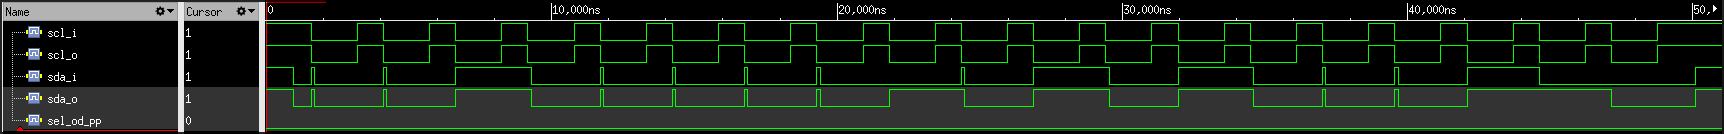
\includegraphics[width=\textwidth]{i2c_write/i2c_write.png}};
		\begin{scope}[shift={(wave.south west)},
				x={($(wave.south east)-(wave.south west)$)},
				y={($(wave.north west)-(wave.south west)$)}]
			\draw[window] (0.154,-0.14) rectangle (0.191,1.14);
			\draw[window] (0.196,-0.14) rectangle (0.570,1.14);
			\draw[window] (0.575,-0.14) rectangle (0.942,1.14);
			\draw[window] (0.947,-0.14) rectangle (1.000,1.14);
			\node[condtag, anchor=south] at (0.1725,1.16) {S};
			\node[condtag, anchor=south] at (0.383,1.16) {Address Phase};
			\node[condtag, anchor=north] at (0.383,-0.16) {0x50, RnW = Write};
			\node[condtag, anchor=south] at (0.7585,1.16) {Data Phase};
			\node[condtag, anchor=north] at (0.7585,-0.16) {0x51};
			\node[condtag, anchor=south] at (0.9735,1.16) {P};
		\end{scope}
	\end{tikzpicture}
